% --------------------------------------------------
% DOCUMENT CLASS
% --------------------------------------------------

\documentclass[../quali_slides.tex]{subfiles}

\begin{document}

% --------------------------------------------------
% RESULTS
% --------------------------------------------------

\section{Results}

% --------------------------------------------------
% MAIN RESULTS
% --------------------------------------------------

\begin{frame}{Main Results}
	
	\begin{itemize}
		
		\item Given the Regional DSGE model, a region more capital intensive ($\alpha_{\eta}$) and with a higher production technology level ($Z_{A\eta}$) is more sensitive to a monetary shock:
		
		\begin{align}
			\alpha_{1}>\alpha_{2} \land Z_{A1}>Z_{A2} \implies \Delta \mathbf{X}_{1} > \Delta \mathbf{X}_{2}
		\end{align}
		
		\item The responses are different in intensity, bot not in direction.
		
	\end{itemize}
	
\end{frame}

% --------------------------------------------------
% IMPULSE RESPONSE FUNCTIONS
% --------------------------------------------------

\begin{frame}{Impulse Response Functions}

\center Positive Monetary Policy Shock of 1\%

\begin{figure}[h!]
	\centering
	\begin{subfigure}[b]{0.45\textwidth}
		\centering
		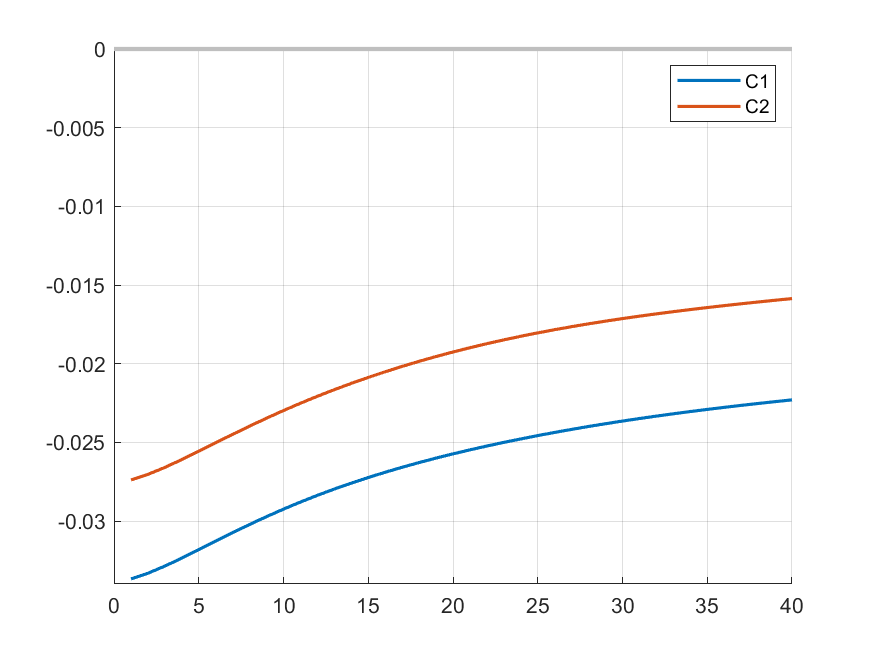
\includegraphics[width=\textwidth]{plots/plot_eM_pos_C1_C2}
		\caption{\scriptsize Consumption}
		\label{fig:plot_eM_pos_C1_C2}
	\end{subfigure}
	\hspace*{0.3cm}
	\begin{subfigure}[b]{0.45\textwidth}
		\centering
		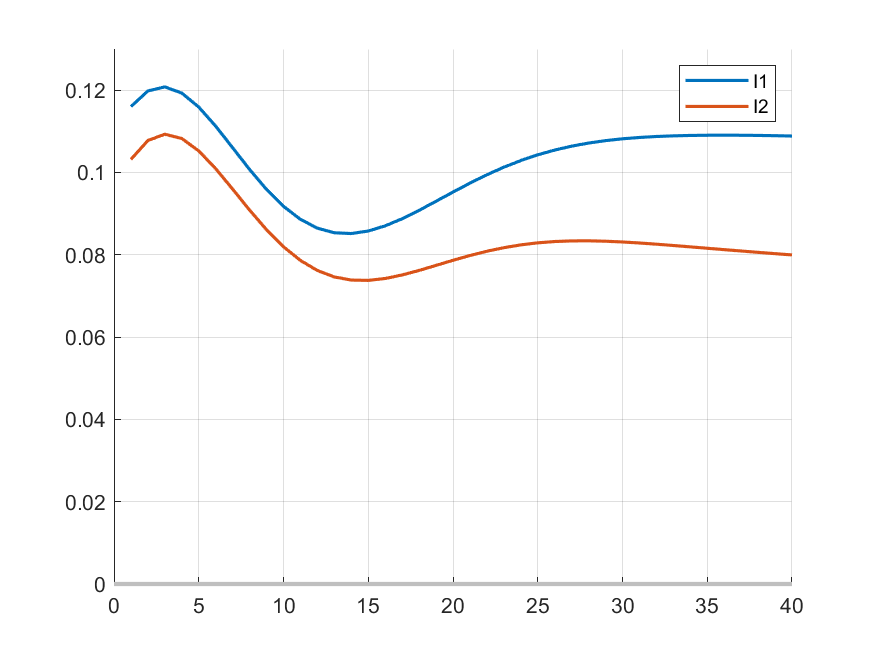
\includegraphics[width=\textwidth]{plots/plot_eM_pos_I1_I2}
		\caption{\scriptsize Investment}
		\label{fig:plot_eM_pos_I1_I2}
	\end{subfigure}
\end{figure}

\end{frame}

% --------------------------------------------------
% IMPULSE RESPONSE FUNCTIONS
% --------------------------------------------------

\begin{frame}{Impulse Response Functions}

\center Positive Monetary Policy Shock of 1\%
	
	\begin{figure}[h!]
		\centering
		\begin{subfigure}[b]{0.45\textwidth}
			\centering
			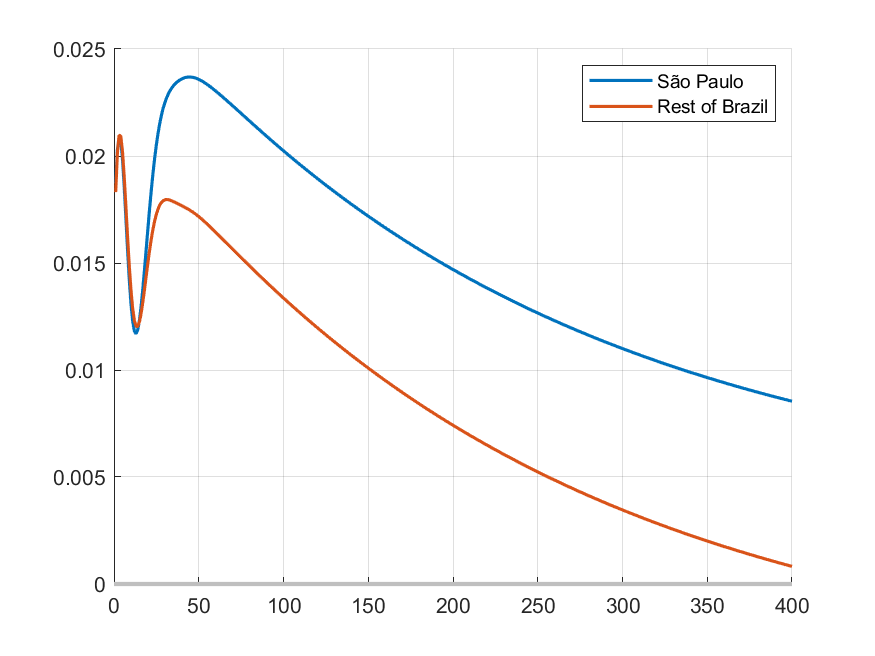
\includegraphics[width=\textwidth]{plots/plot_eM_pos_Y1_Y2}
			\caption{\scriptsize Production}
			\label{fig:plot_eM_pos_Y1_Y2}
		\end{subfigure}
		\hspace*{0.3cm}
		\begin{subfigure}[b]{0.45\textwidth}
			\centering
			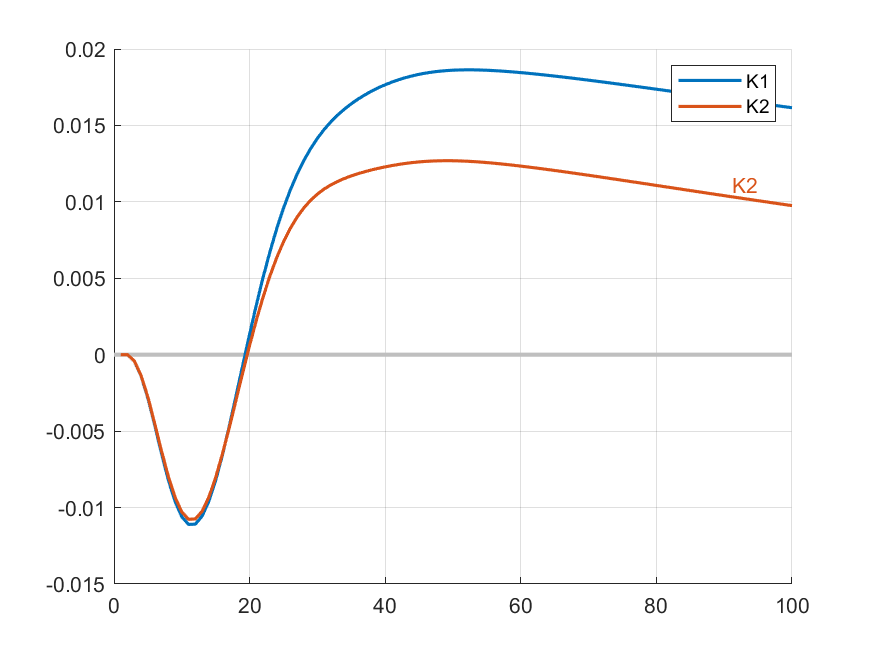
\includegraphics[width=\textwidth]{plots/plot_eM_pos_K1_K2}
			\caption{\scriptsize Capital}
			\label{fig:plot_eM_pos_K1_K2}
		\end{subfigure}
	\end{figure}
	
\end{frame}

% --------------------------------------------------
% IMPULSE RESPONSE FUNCTIONS
% --------------------------------------------------

\begin{frame}{Impulse Response Functions}

\center Positive Monetary Policy Shock of 1\%
	
	\begin{figure}[h!]
		\centering
		\begin{subfigure}[b]{0.45\textwidth}
			\centering
			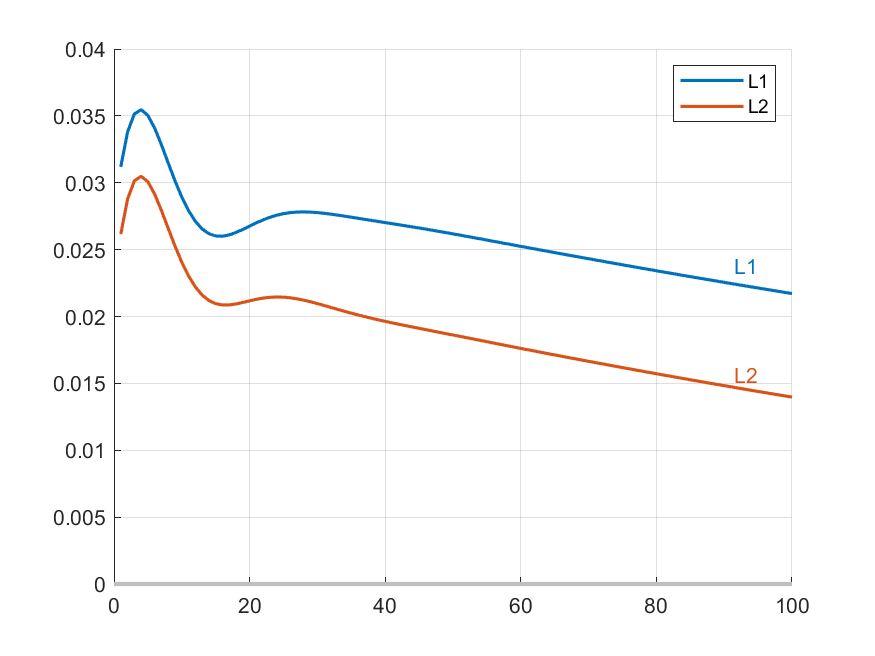
\includegraphics[width=\textwidth]{plots/plot_eM_pos_L1_L2}
			\caption{\scriptsize Labor}
			\label{fig:plot_eM_pos_L1_L2}
		\end{subfigure}
		\hspace*{0.3cm}
		\begin{subfigure}[b]{0.45\textwidth}
			\centering
			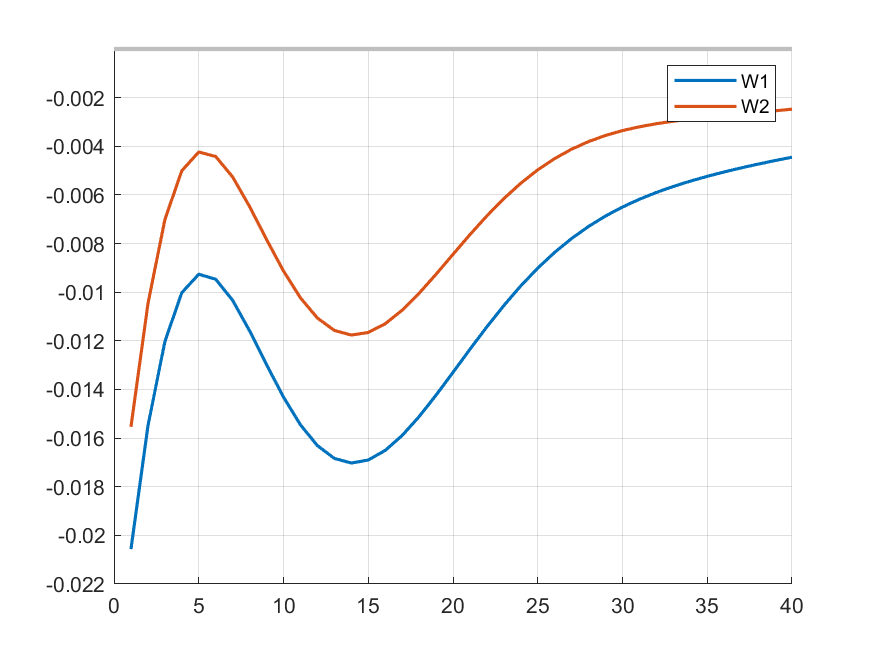
\includegraphics[width=\textwidth]{plots/plot_eM_pos_W1_W2}
			\caption{\scriptsize Wages}
			\label{fig:plot_eM_pos_W1_W2}
		\end{subfigure}
	\end{figure}
	
\end{frame}

% --------------------------------------------------
% IMPULSE RESPONSE FUNCTIONS
% --------------------------------------------------

\begin{frame}{Impulse Response Functions}

\center Positive Monetary Policy Shock of 1\%
	
	\begin{figure}[h!]
		\centering
		\begin{subfigure}[b]{0.45\textwidth}
			\centering
			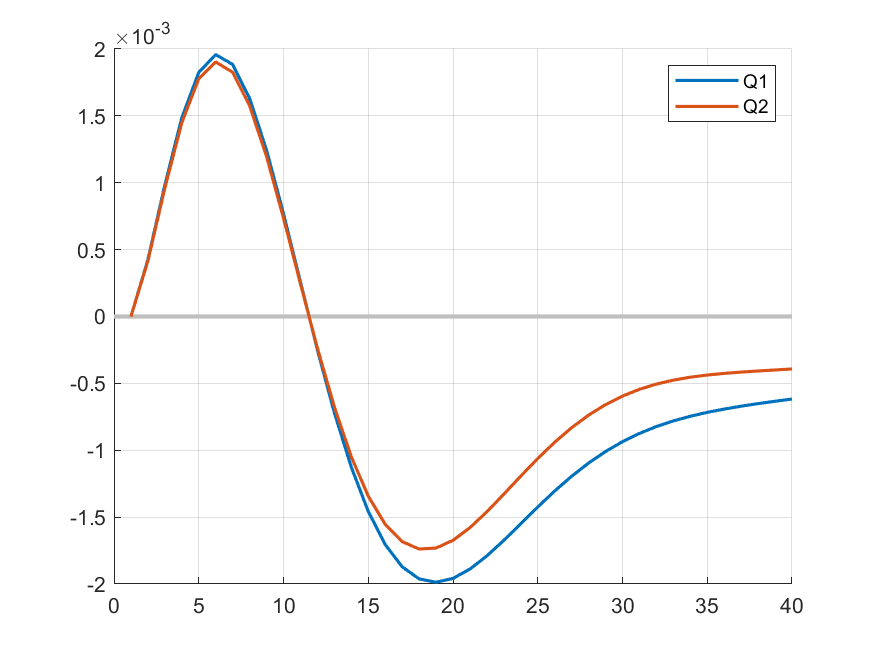
\includegraphics[width=\textwidth]{plots/plot_eM_pos_Q1_Q2}
			\caption{\scriptsize Consumer Price Level}
			\label{fig:plot_eM_pos_Q1_Q2}
		\end{subfigure}
		\hspace*{0.3cm}
		\begin{subfigure}[b]{0.45\textwidth}
			\centering
			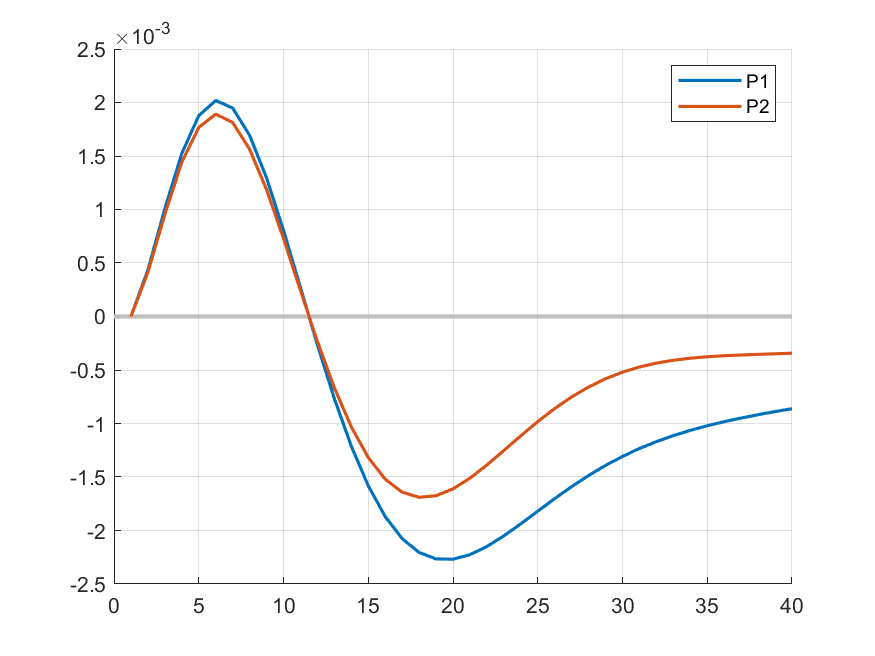
\includegraphics[width=\textwidth]{plots/plot_eM_pos_P1_P2}
			\caption{\scriptsize Price Level}
			\label{fig:plot_eM_pos_P1_P2}
		\end{subfigure}
	\end{figure}
	
\end{frame}

% --------------------------------------------------
% FINAL REMARKS
% --------------------------------------------------

\section{Final Remarks}

\begin{frame}{Final Remarks}
	
	\begin{itemize}
		
		\item The national wide interest rate may not have the same effectiveness across all regions of a country with different economic structures.
		
		\item Other instruments may be applied in conjunction to achieve the desired objectives of public policies.
		
		\item Future challenges include augmenting the model with additional elements to better describe Brazilian regions.
		
	\end{itemize}
	
\end{frame}

\end{document}